\documentclass[11pt]{article}

\usepackage{amsmath}
\usepackage{amssymb}
\usepackage{amsfonts}
\usepackage{mathtools}

\usepackage[thmmarks, amsmath]{ntheorem}

\usepackage{graphicx}
\usepackage{float}

\usepackage{tikz-cd}

\usepackage{diffcoeff}
\diffdef{}{op-symbol=\mathrm{d},op-order-sep=0mu}

\usepackage{cancel}
\usepackage{interval}

\usepackage{enumitem}

%\usepackage{cite}

\usepackage[utf8]{inputenc}
\usepackage[portuguese]{babel}
\usepackage[margin=3cm]{geometry}

%\setlist[enumerate,1]{label=\alph*)}

\title{Handout: Apresentação 1\\
Introdução a Persistence Homology}
\author{Duarte Maia}
%\date{}

\theorembodyfont{\upshape}
\theoremseparator{.}
\newtheorem{theorem}{Teorema}
\newtheorem{prop}{Prop}
\renewtheorem*{prop*}{Prop}
\newtheorem{lemma}{Lema}
\theoremsymbol{\ensuremath{\square}}
\newtheorem{definition}{Definição}
\newtheorem{ex}{Exemplo}

\theoremstyle{nonumberplain}
\theoremheaderfont{\itshape}
\theorembodyfont{\upshape}
\theoremseparator{:}
\theoremsymbol{\ensuremath{\blacksquare}}
\newtheorem{proof}{Proof}

\newcommand{\R}{\mathbb{R}}
\newcommand{\C}{\mathbb{C}}
\newcommand{\Z}{\mathbb{Z}}
\newcommand{\FF}{\mathbb{F}}

\newcommand{\PP}{\mathbb{P}}
\newcommand{\LL}{\mathrm{L}}
\renewcommand{\AA}{\mathrm{A}}
\newcommand{\BB}{\mathrm{B}}


\newcommand{\CF}{\mathrm{CF}}
\newcommand{\HF}{\mathrm{HF}}

\newcommand{\I}{\mathrm{i}}
\newcommand{\e}{\mathrm{e}}

\newcommand{\Ix}{\mathop{\mathrm{I\mkern0.7mu x}}}
%\newcommand{\Ix}{\mathop{\mathrm{ix}}}


\newcommand{\id}{\mathrm{id}}


\DeclareMathOperator{\inte}{int}
\DeclareMathOperator{\codim}{codim}
\newcommand{\grad}{\nabla}
\newcommand{\into}{\mathbin{\lrcorner}}

\DeclarePairedDelimiter{\norm}{\lvert}{\rvert}
\DeclarePairedDelimiter{\Norm}{\lVert}{\rVert}
\DeclarePairedDelimiter{\abs}{\lvert}{\rvert}
\DeclarePairedDelimiter{\braket}{\langle}{\rangle}


\begin{document}

\shorthandoff{"}

\maketitle

\section{Persistence Modules}

Existem construções que associam espaços vetoriais a objetos geométricos. O exemplo mais conveniente é a homologia de uma variedade $M$ com escalares num corpo $\FF$. Este objeto dá-nos informação `global' da variedade.

Suponha-se agora que temos uma função de Morse $f$ numa variedade $M$. Podemos ver $M$ como sendo `construido de baixo para cima' e podemos usar isso para calcular a Homologia (de Morse) de $M$. Essa homologia dá informação global sobre a variedade, mas uma modificação elementar dá a chamada `Homologia de Morse filtrada' de $M$. Em suma, consideramos os espaços $M_t = f^{-1}(-\infty, t)$ e calculamos a sua homologia $H_*(M_t)$. Isto é um espaço vetorial que depende de $t$ e nos dá informação topológica sobre a variedade, mais do que a homologia total. Por exemplo, a homologia permite-nos detetar buracos no espaço, mas a homologia filtrada dá-nos noção de onde eles se situam. Ver figura \ref{mt1}.

\begin{figure}[h]
\centering
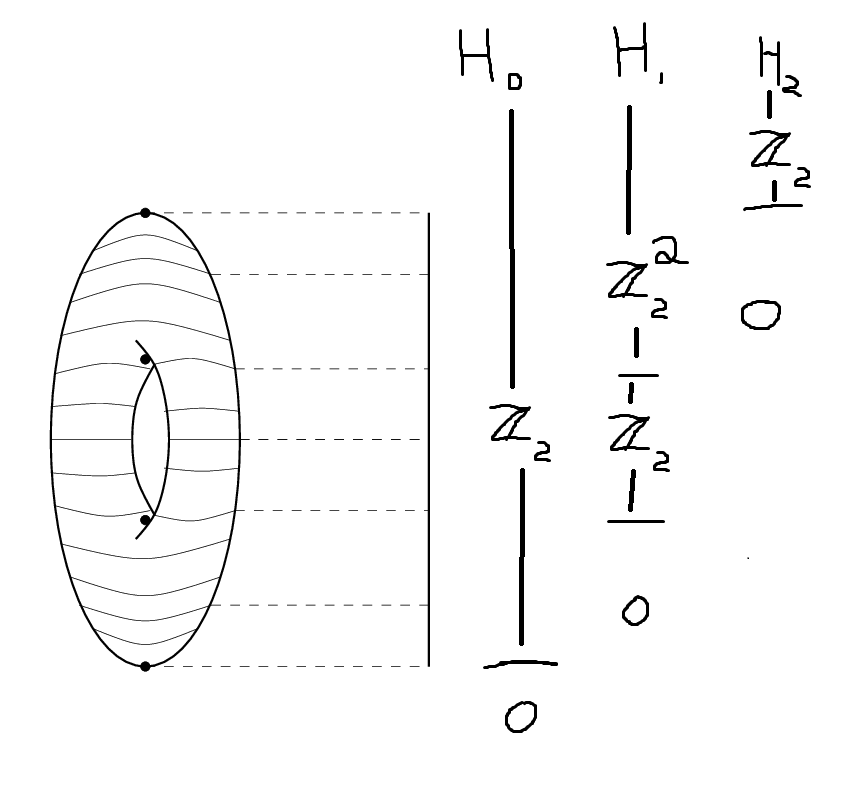
\includegraphics[width=7cm]{mt1}
\caption{A homologia filtrada do toro}\label{mt1}
\end{figure}

A homologia filtrada de $M$ diz-nos sensivelmente a que altura se situam os buracos, e também nos permite relacioná-los. De facto, as inclusões $M_t \hookrightarrow M_s$, para $t \leq s$, induzem mapas naturais nas homologias
\begin{equation}
\pi_{ts} \colon H_*(M_t) \to H_*(M_s).
\end{equation}

Isto motiva então a seguinte noção:

\begin{definition}[Persistence module]
Um \emph{persistence module} é uma coleção $\{V_t\}_{t \in \R}$ de espaços vetoriais de dimensão finita sobre um corpo $\FF$, juntamente com mapas
\begin{equation}
\pi_{ts} \colon V_t \to V_s, \quad t \leq s,
\end{equation}
tais que $\pi_{tt} = \id_{V_t}$ e o seguinte diagrama comuta:
\begin{equation}
% https://tikzcd.yichuanshen.de/#N4Igdg9gJgpgziAXAbVABwnAlgFyxMJZABgBpiBdUkANwEMAbAVxiRADUB9HEAX1PSZc+QigCM5KrUYs2XBP0HY8BIgCZJ1es1aIOnAE58pMKAHN4RUADMDEALZIyIHBCQTpOtgB1vaLJzAOHC8fAIgtg7u1K5IGp6yer7+gXAGoYoRdo6IzrGI8QBGMGBQSADMztqJIMkBQSEg1HAAFljWPIgAtGq8FLxAA
\begin{tikzcd}
V_t \arrow[r, "\pi_{ts}"] \arrow[rr, "\pi_{ts}", bend left, shift left=2] & V_s \arrow[r, "\pi_{sr}"] & V_r
\end{tikzcd}
\end{equation}
\end{definition}

\begin{ex}\label{homfil}
Dada uma variedade $M$ e uma função de Morse $f$, podemos considerar os vários persistence modules associados às homologias filtradas de $M$. Ou seja, define-se (para $* \in \Z$)
\begin{equation}
V_t = H_*(f^{-1}(-\infty, t)),
\end{equation}
e $\pi_{ts}$ para $t<s$ os mapas induzidos pelas inclusões.
\end{ex}

\section{Códigos de Barras}

Parte do benefício de espaços vetoriais (em prole de, por exemplo, anéis ou grupos) é que um espaço vetorial é unicamente determinado por um número: a sua dimensão. É possível tentar reduzir um persistence module de forma semelhante, definindo por exemplo $n_t = \dim V_t$. No entanto, isso perde toda a informação sobre como os $V_t$ se relacionam uns com os outros.

Um código de barras permite guardar a informação sobre a dimensão dos $V_t$, para além de permitir perceber a relação entre os espaços.

\begin{ex}\label{exxy}
Considere-se os dois seguintes espaços $X$ e $Y$ e as suas homologias filtradas em grau 1:
\begin{figure}[H]
\centering
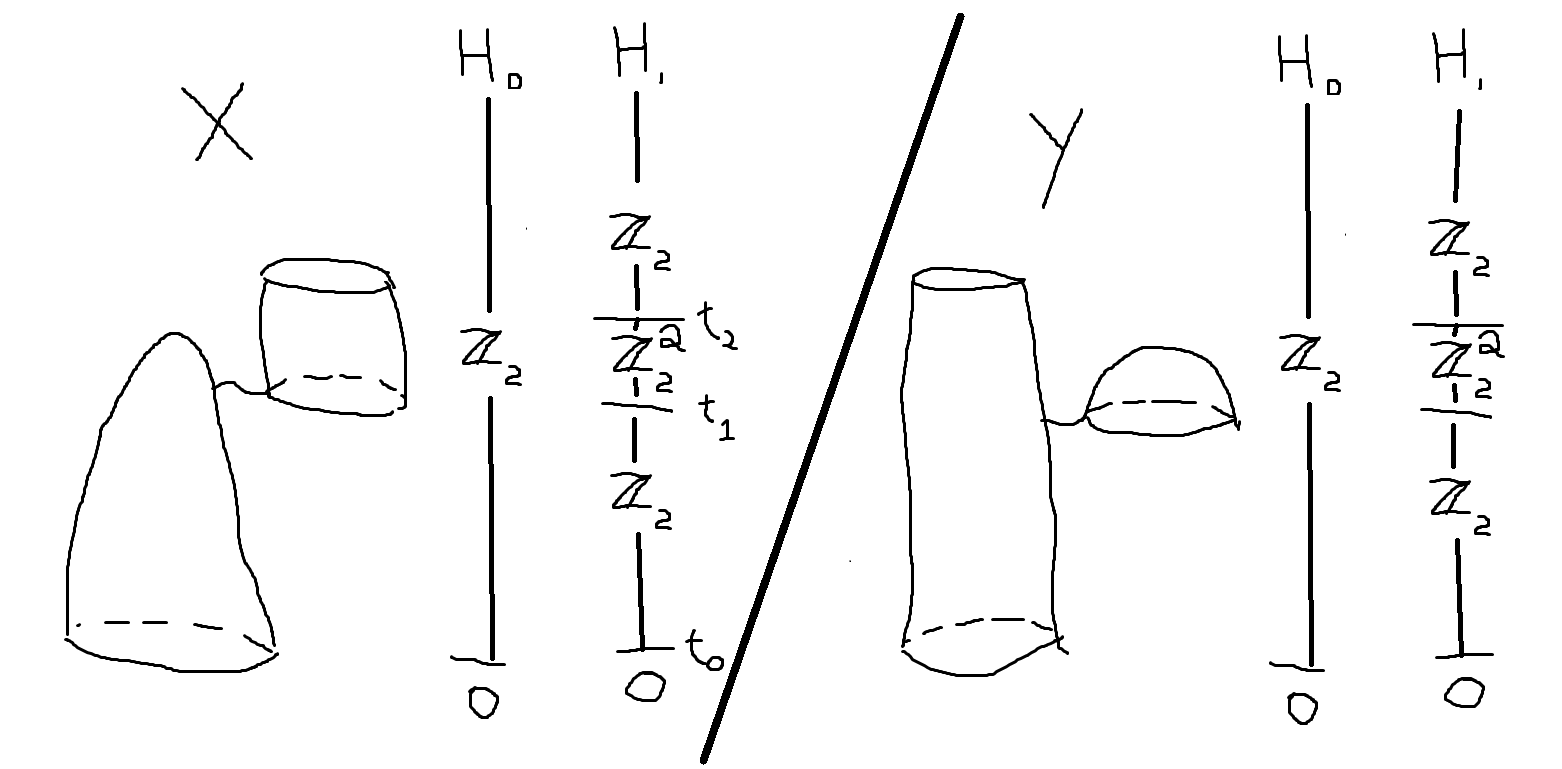
\includegraphics[height=5cm]{mt2}
\caption{As homologias filtradas de dois espaços $X$ e $Y$}\label{mt2}
\end{figure}

A homologia filtrada em grau 1 de $X$ e $Y$ é a mesma, e contam ambos a mesma história. Em $t = t_0$ é criado um componente conexo que contém um ciclo não-contrátil. Em $t = t_1$ é criado outro buraco no mesmo componente conexo, mas um dos dois buracos é fechado em $t = t_2$.

Pelo outro lado, o persistence module $(V,\pi)$ associado a $X$ (em grau 1) é distinto daquele $(W,\pi)$ associado a $Y$, porque estes conseguem detetar qual dos buracos é fechado em $t_2$. Mais concretamente, sejam $t_{0.5}$, $t_{1.5}$ e $t_{2.5}$ tais que
\[t_0 < t_{0.5} < t_1 < t_{1.5} < t_2 < t_{2.5}.\]

Seja $a$ um gerador de $V_{t_{0.5}}$. Então, $a' = \pi_{t_{0.5} t_{1.5}}(a)$ é um elemento (não-nulo) de $V_{t_{1.5}}$, e como este tem dimensão dois, concluímos que existe algum $b \in V_{t_{1.5}}$ tal que $V_{t_{1.5}}$ é gerado por $a'$ e $b$. Estes dois representam ciclos não-triviais em $X_{t_{1.5}}$. Agora, o que é interessante é considerar a imagem destes elementos sob $\pi_{t_{1.5} t_{2.5}}$. De facto, a imagem de $a'$ é nula, enquanto que $b$ `sobrevive'. Isto diz-nos que o ciclo que se fecha é precisamente o que foi o primeiro a abrir-se.

No $W$ as coisas estão trocadas. Se construirmos $a, a', b$ da mesma forma, obtemos que a imagem sob $\pi_{t_{1.5} t_{2.5}}$ de $b$ é nula e a de $a'$ não. Isso indica que, em $Y$, o ciclo que sobrevive até o infinito foi o primeiro a fechar-se.
\end{ex}

\begin{ex}
O exemplo anterior pode ser modificado para obter uma versão mais flagrante do mesmo fenómeno. Considere-se o caso limite em que $t_2 = t_1$, em que $Y$ é apenas um cilindro e $X$ consiste numa `taça ao contrário' com um círculo colado à sua base. Então, em ambos os casos as homologias filtradas vêm apenas que, para todo o $t > t_0$, $X$ e $Y$ têm exatamente um buraco unidimensional. No entanto, a anomalia é detetada pelo persistence module de $X$, para o qual $\pi_{t_{0.5} t_{2.5}}$ é o mapa nulo. Em certo sentido, o persistence module consegue detetar que o $\Z_2$ entre $t_0$ e $t_1$ não representa o mesmo ciclo que aquele entre $t_2$ e $+\infty$.
\end{ex}

Um código de barras pode ser visto como guardando informação sobre bases dos $V_t$. A figura \ref{bc1} mostra os códigos de barras correspondentes a $X$ e $Y$.
\begin{figure}[H]
\centering
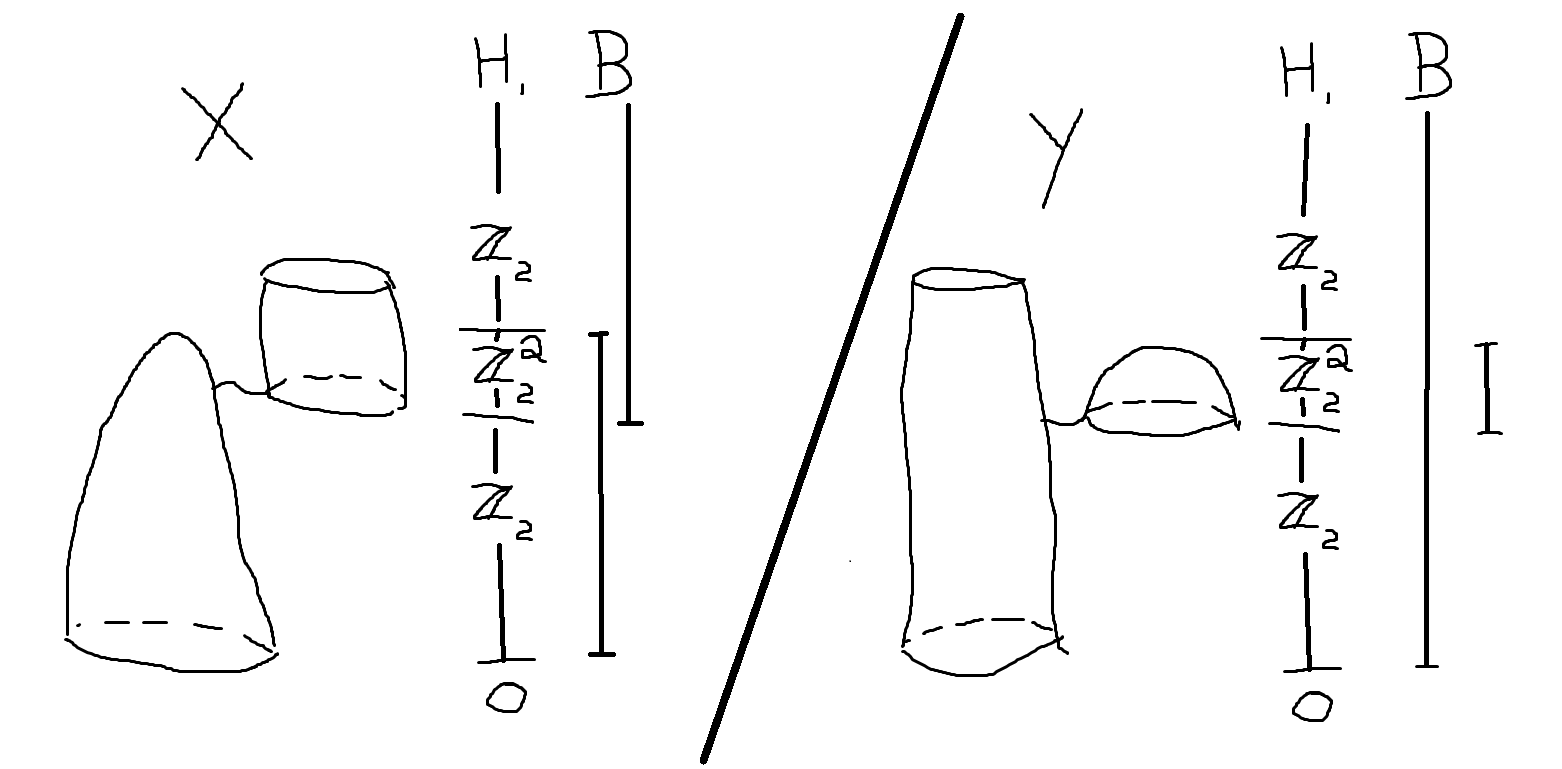
\includegraphics[height=5cm]{bc1}
\caption{Códigos de barras das homologias filtradas (grau 1)}\label{bc1}
\end{figure}

Nesta figura é possível ver que os códigos de barras conseguem perceber qual dos ciclos se torna num ciclo contrátil. Podemos ver uma das barras como correspondendo ao ciclo $a$ do exemplo \ref{exxy} e a outra ao ciclo $b$.

\begin{definition}[Código de barras]
Um código de barras é um multiconjunto\footnote{Podem haver barras repetidas} finito de intervalos da forma $\linterval a b$, com $-\inf < a < b \leq +\infty$.
\end{definition}

\begin{definition}
Seja $B = \{I_1, \dots, I_k\}$ um código de barras. Definimos o \emph{persistence module associado a $B$}, denominado $\FF(B)$, da seguinte forma:
\begin{gather}
V_t = \braket{\,i \mid t \in I_i}_\FF,\\
\pi_{ts}(i) = \begin{cases} i, & s \in I_i,\\ 0 & \text{c.c.} \end{cases}
\end{gather}
\end{definition}

\begin{ex}
Considere-se o código de barras
\begin{equation}
B = \{I_1, I_2, I_3, I_4\} = \{\,\rinterval{-\infty}0, \linterval{-\infty}3, \linterval 0 1, \ointerval 4 {+\infty} \,\},
\end{equation}
representado na figura \ref{bc2}, juntamente com os $V_t$ associados.

\begin{figure}[H]
\centering
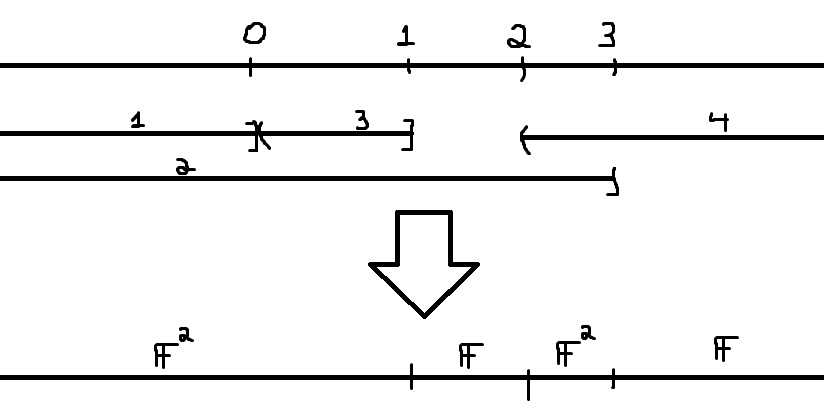
\includegraphics[height=5cm]{bc2}
\caption{O código de barras $B$ e os espaços vetoriais $V_t$ associados}\label{bc2}
\end{figure}

Como se pode ver, para $t \in \R$, $V_t$ é um espaço vetorial com dimensão igual ao números de barras em $t$. Não representado na figura estão os mapas $\pi$.
\begin{enumerate}
\item Entre quaisquer dois elementos adjacentes de $\{-\infty,0,1,2,3,+\infty\}$, os mapas $\pi$ são a identidade,
\item Os mapas $\pi_{1-\varepsilon, 1+\varepsilon}$ são a projeção num dos componentes,
\item Idem para $\pi_{3-\varepsilon, 3+\varepsilon}$,
\item Os mapas $\pi_{2-\varepsilon,2+\varepsilon}$ consistem numa inclusão de $\FF$ em $\FF^2$, mas especificamente \emph{no núcleo de $\pi_{2+\varepsilon, 3+\varepsilon}$!}
\item Os mapas $\pi_{2-\varepsilon,3+\varepsilon}$ são nulos,
\item Os mapas $\pi_{-\varepsilon,+\varepsilon}$ são da forma $(x,y) \mapsto (x,0)$.
\end{enumerate}
\end{ex}

O \emph{Normal Form Theorem} estabelece que $B \mapsto \FF(B)$ é uma correspondência biunívoca entre códigos de barras e persistence modules, assumindo algumas hipóteses de finitude.

\begin{definition}
Um persistence module $(V,\pi)$ diz-se \emph{de tipo finito} se satisfaz as seguintes condições.
\begin{enumerate}[label=\roman*)]
\item\label{pm1} Para todos os valores de $t \in \R$ exceto um número finito, existe uma vizinhança $U$ de $t$ tal que $\pi_{rs}$ é um isomorfismo para todos os $r,s \in U$,
\item\label{pm2} \textit{(Semicontinuidade)} Para todo o $t \in \R$ existe $\varepsilon > 0$ tal que $\pi_{rt}$ é um isomorfismo, para $t-\varepsilon < r < t$.
\end{enumerate}

É fácil mostrar a partir de \ref{pm1} que $V_t$ muda (a menos de isomorfismo) um número finito de vezes. Consequentemente, para $t$ perto o suficiente de $+\infty$, $V_t$ é constante (a menos de isomorfismo), pelo que todos os $V_t$ (para $t$ grande) podem ser identificados simultaneamente com o mesmo espaço vetorial, que chamaremos $V_+$. O mesmo poderia ser feito para $t$ próximo de $-\infty$, mas adicionamos a seguinte hipótese:

\begin{enumerate}[resume*]
\item\label{pm3} Para $t$ próximo o suficiente de $-\infty$, $V_t = 0$.
\end{enumerate}
\end{definition}

Nota: É trivial verificar que $\FF(B)$ é de tipo finito.

\begin{theorem}[Normal Form Theorem]
Qualquer persistence module de tipo finito é da forma $\FF(B)$ para algum código de barras $B$. Para mais, se $\FF(B)$ é isomorfo a $\FF(B')$, então $B = B'$.
\end{theorem}

\section{Exemplo: Funções de Morse}

Com base no NFT é possível associar a uma função de Morse $f$ numa variedade compacta $M$ um código de barras único, usando o exemplo \ref{homfil}, da homologia filtrada.

\begin{lemma}
O persistence module associado à homologia filtrada de $M$ (de grau $* \in \Z$) é de tipo finito.
\end{lemma}

\begin{proof}
Verificamos as propriedades uma a uma. A propriedade \ref{pm3} é a mais fácil: Como $M$ é compacto, por Weierstrass $f$ tem mínimo. Para $t$ menor que esse mínimo, $f^{-1}(-\infty,t) = \emptyset$, que tem homologia nula.

A propriedade \ref{pm1} resume-se aos dois factos clássicos:
\begin{enumerate}
\item Os pontos críticos de uma função de Morse numa variedade compacta são isolados, (\cite{milnor}, Corollary 2.3, ou \cite{audin}, Corollary 1.3.2) e portanto em número finito,
\item Se não existe nenhum valor crítico entre $t_1$ e $t_2$ (inclusive), a inclusão induz um isomorfismo entre a homologia dos sub-level sets de $t_1$ e $t_2$ (\cite{milnor}, Theorem 3.1).
\end{enumerate}

Consequentemente, dado um valor regular $t$, os quais são todos exceto um número finito, é possível encontrar uma vizinhança de $t$ de valores também regulares, para os quais os $\pi$ são isomorfismos.

Finalmente, o seguinte lema justifica a propriedade \ref{pm2}:

\begin{lemma}
Seja $f$ é uma função de Morse em $M$, uma variedade compacta. Então, se $t_1 < t_2$ são tais que o intervalo $\linterval{t_1}{t_2}$ não contém nenhum valor crítico de $f$, temos que $f^{-1}(-\infty,t_1)$ é uma retração por deformação de $f^{-1}(-\infty, t_2)$. Consequentemente, a inclusão do primeiro no segundo induz um isomorfismo em homologia.
\end{lemma}

A demonstração pode ser esboçada com ideias muito semelhantes às usadas em \cite{milnor}, Theorem 3.2.

Isto conclui a demonstração de que a homologia filtrada de $M$ tem tipo finito.
\end{proof}

\begin{definition}
Seja $f$ uma função de Morse numa variedade compacta $M$. Definimos $B_*(f)$ como sendo o código de barras associado ao persistence module $V_t = H_*(f^{-1}(-\infty,t)$, e definimos o \emph{código de barras total de $f$} como sendo a união dos $B_*(f)$.
\end{definition}

\begin{ex}
Na figura \ref{mt1} encontra-se a homologia filtrada do toro. Computações elementares mostram que as funções $\pi$ são sempre as inclusões, pelo que o código de barras da função de Morse representada é a da figure \ref{bctorus}
\begin{figure}[H]
\centering
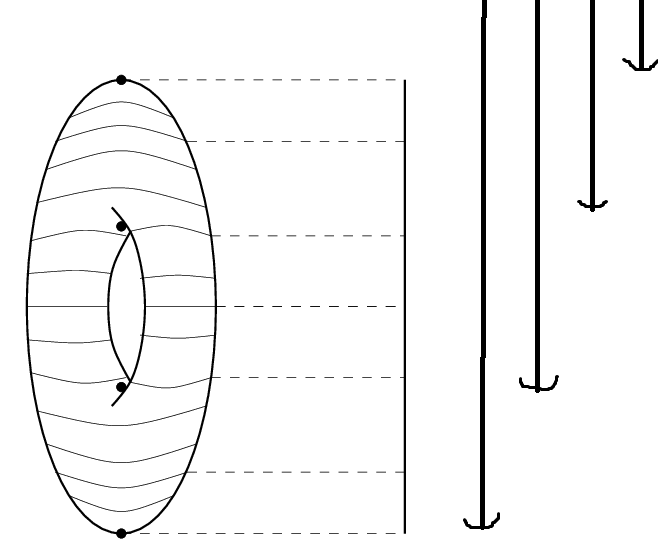
\includegraphics[height=5cm]{bctorus}
\caption{Código de barras total do toro} \label{bctorus}
\end{figure}
\end{ex}

\begin{ex}
A figura \ref{bcspheres} ilustra o código de barras da esfera com duas funções de Morse distintas.

Em ambos os casos temos uma barra de início no mínimo e uma de início no máximo da função de Morse. No entanto, devido ao amolgamento, a esfera amolgada tem uma barra finita que provém da homologia 1.
\begin{figure}[H]
\centering
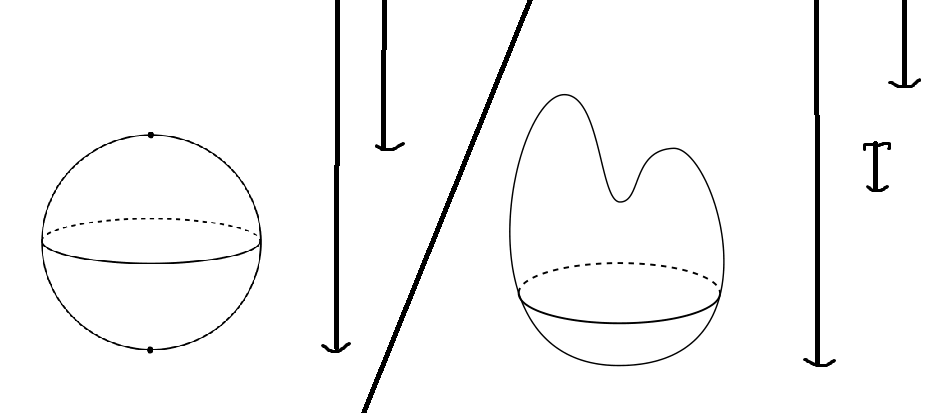
\includegraphics[height=5cm]{bcspheres}
\caption{Código de barras total da esfera e da esfera amolgada} \label{bcspheres}
\end{figure}
\end{ex}

\begin{ex}[Funções em $S^1$]
Seja $f$ uma função de Morse em $S^1$. Existe um algoritmo simples para calcular o código de barras de $f$, que exemplificaremos para uma função `genérica'.

Como estamos em dimensão 1, todos os pontos críticos de $f$ são máximos ou mínimos. Cada mínimo corresponde à criação de uma componente conexa, ou seja, a criação de uma barra em homologia zero. Cada máximo (com a exceção do global) corresponde à junção de dois componentes conexos, e portanto à eliminação de uma barra, sendo apenas necessário determinar qual. Finalmente, o máximo corresponde a `fechar o círculo', que faz com que a homologia de grau 1 passe de 0 a $\FF$.

Isto permite-nos já calcular códigos de barras simples, como na figura \ref{bcs11}.
\begin{figure}[H]
\centering
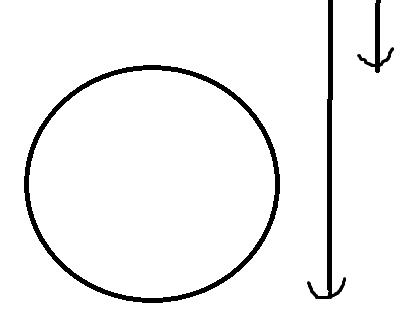
\includegraphics[height=4cm]{bcs11}
\caption{Código de barras total de $S^1$} \label{bcs11}
\end{figure}

Para calcular códigos de barras mais complexos, é preciso determinar como se processa a eliminação de barras. Para isso, considere-se o exemplo simples do círculo com uma mossa; ver figura \ref{bcs12}.
\begin{figure}[H]
\centering
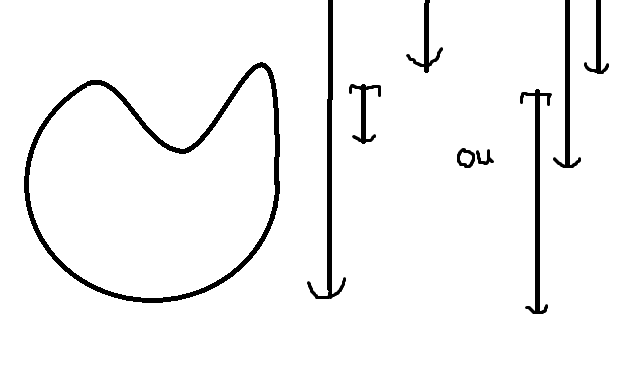
\includegraphics[height=4cm]{bcs12}
\caption{Alternativas para o código de barras de $S^1$ com uma mossa} \label{bcs12}
\end{figure}

Estão representadas as duas possibilidades para o código de barras. Para determinar qual destas se verifica, basta olhar para o mapa $\pi_{ts}$, em que $t$ é um valor entre o mínimo global de $f$ e o mínimo local e $s$ é um valor superior ao máximo. Este mapa não se anula, pois um gerador da homologia de $f^{-1}(-\infty,t)$ não se anula quando visto como um elemento da homologia de $S^1$. Consequentemente, a alternativa da direita não pode acontecer, pois do ponto de vista dessa o mapa $\pi_{ts}$ é nulo. Logo, o código de barras deste $S^1$ é o código de barras da esquerda.

Este exemplo é instrutivo porque nos permite perceber melhor que elementos (das bases de $H_*$) são representados pelas barras. Sejam $a$, $b$ e $c$ as barras da esquerda para a direita.

A barra $a$ representa um elemento da homologia de grau zero de qualquer $f^{-1}(-\infty, t)$, para $t > \min f$. Por exemplo, o ponto minimizante de $f$.

A barra $c$ representa um ciclo não-trivial da homologia de grau 1 de $S^1$, por exemplo uma volta ao círculo.

A barra $b$ é ligeiramente mais complicada. Ela representa um elemento não-nulo da homologia de grau zero de $M_t = f^{-1}(-\infty, t)$, onde $t$ é um valor entre o mínimo local e o máximo global. Ora, $M_t$ tem dois componentes conexos, $C_1$ e $C_2$, e $a$ representa um ponto em $C_1$, pelo que é tentador que $b$ seja representado por um ponto em $C_2$. No entanto, essa conjetura não se pode verificar, pois se fosse esse o caso ter-se-ia $\pi_{ts}(b) = a \neq 0$, em que $s > \max f$. No entanto, como a barra correspondente a $b$ termina após o máximo local, é necessário que $\pi_{ts}(b) = 0$. Assim sendo, na verdade $b$ representa um elemento da homologia como por exemplo
\[ b = p - a \text{, onde $p$ é o mínimo local.}\]

Este exemplo mostra que os elementos representados por barras nem sempre são triviais.
\end{ex}

\nocite{polterovich}

\bibliographystyle{plain}
\bibliography{bibliography}

\end{document}